% !TEX TS-program = pdflatex
% !TEX root = ../tesi.tex

\chapter{Applicazione}

\section{Obiettivi}
Gli obiettivi di questa ricerca, con l’utilizzo dell’idrofono, sono quelli di evidenziare come il rumore ripreso sul fondo del mare, possa riscontrare problematiche a livello acustico di un certo tipo.
Gli idrofoni vengono utilizzati per misurare il rumore antropogenico, come quello prodotto dalle navi, e il suo impatto sull'ambiente marino, qui in Puglia, è davvero notevole;
La ricerca è la parte fondamentale di questo studio, infatti inizialmente la ricerca si è improntata sulla costruzione di un idrofono, con l'utilizzo di piezoelettrici bilanciati, collegati ad un XRL, con l'utilizzo di una scheda audio e di un computer, per effettuare delle registrazioni. 
In merito ai risultati ottenuti, si sono svolte poi altre ricerche e conclusioni, che hanno portato a conclusioni importanti: 

\begin{itemize}
\item La costruzione di un idrofono più professionale con l'utilizzo di piezoelettrici cilindrici in ceramica\ 
\item l'acquisto di un idrofono professionale tramite aziende specializzate nel settore
\item Ricerca di informazioni e dati dai Centri Nazionali di Ricerca nell'ambito della bioacustica e sopratutto specializzati nel rumore. 
\end{itemize}

Dopo svariate ricerche e consulenze in merito, la giusta scelta e sopratutto quella che avrebbe aiutato nello scopo è stata quella di fare ricerchè in merito a Centri Nazionali di Ricerca, Università, e associazioni specializzate nello studio dell'acqua e sopratutto nel mondo del monitoraggio ambientale marino. 

\section{Ricerca e studi}
Inizialmente la ricerca è stata effettuata su che suono avesse l'acqua. Da questo, il protagonista principale è stato l'idrofono. 
Insieme al mio relatore l'applicazione iniziale è stata quella di costruirne uno per effettuare delle registrazioni.

\begin{figure}[h]
\centering
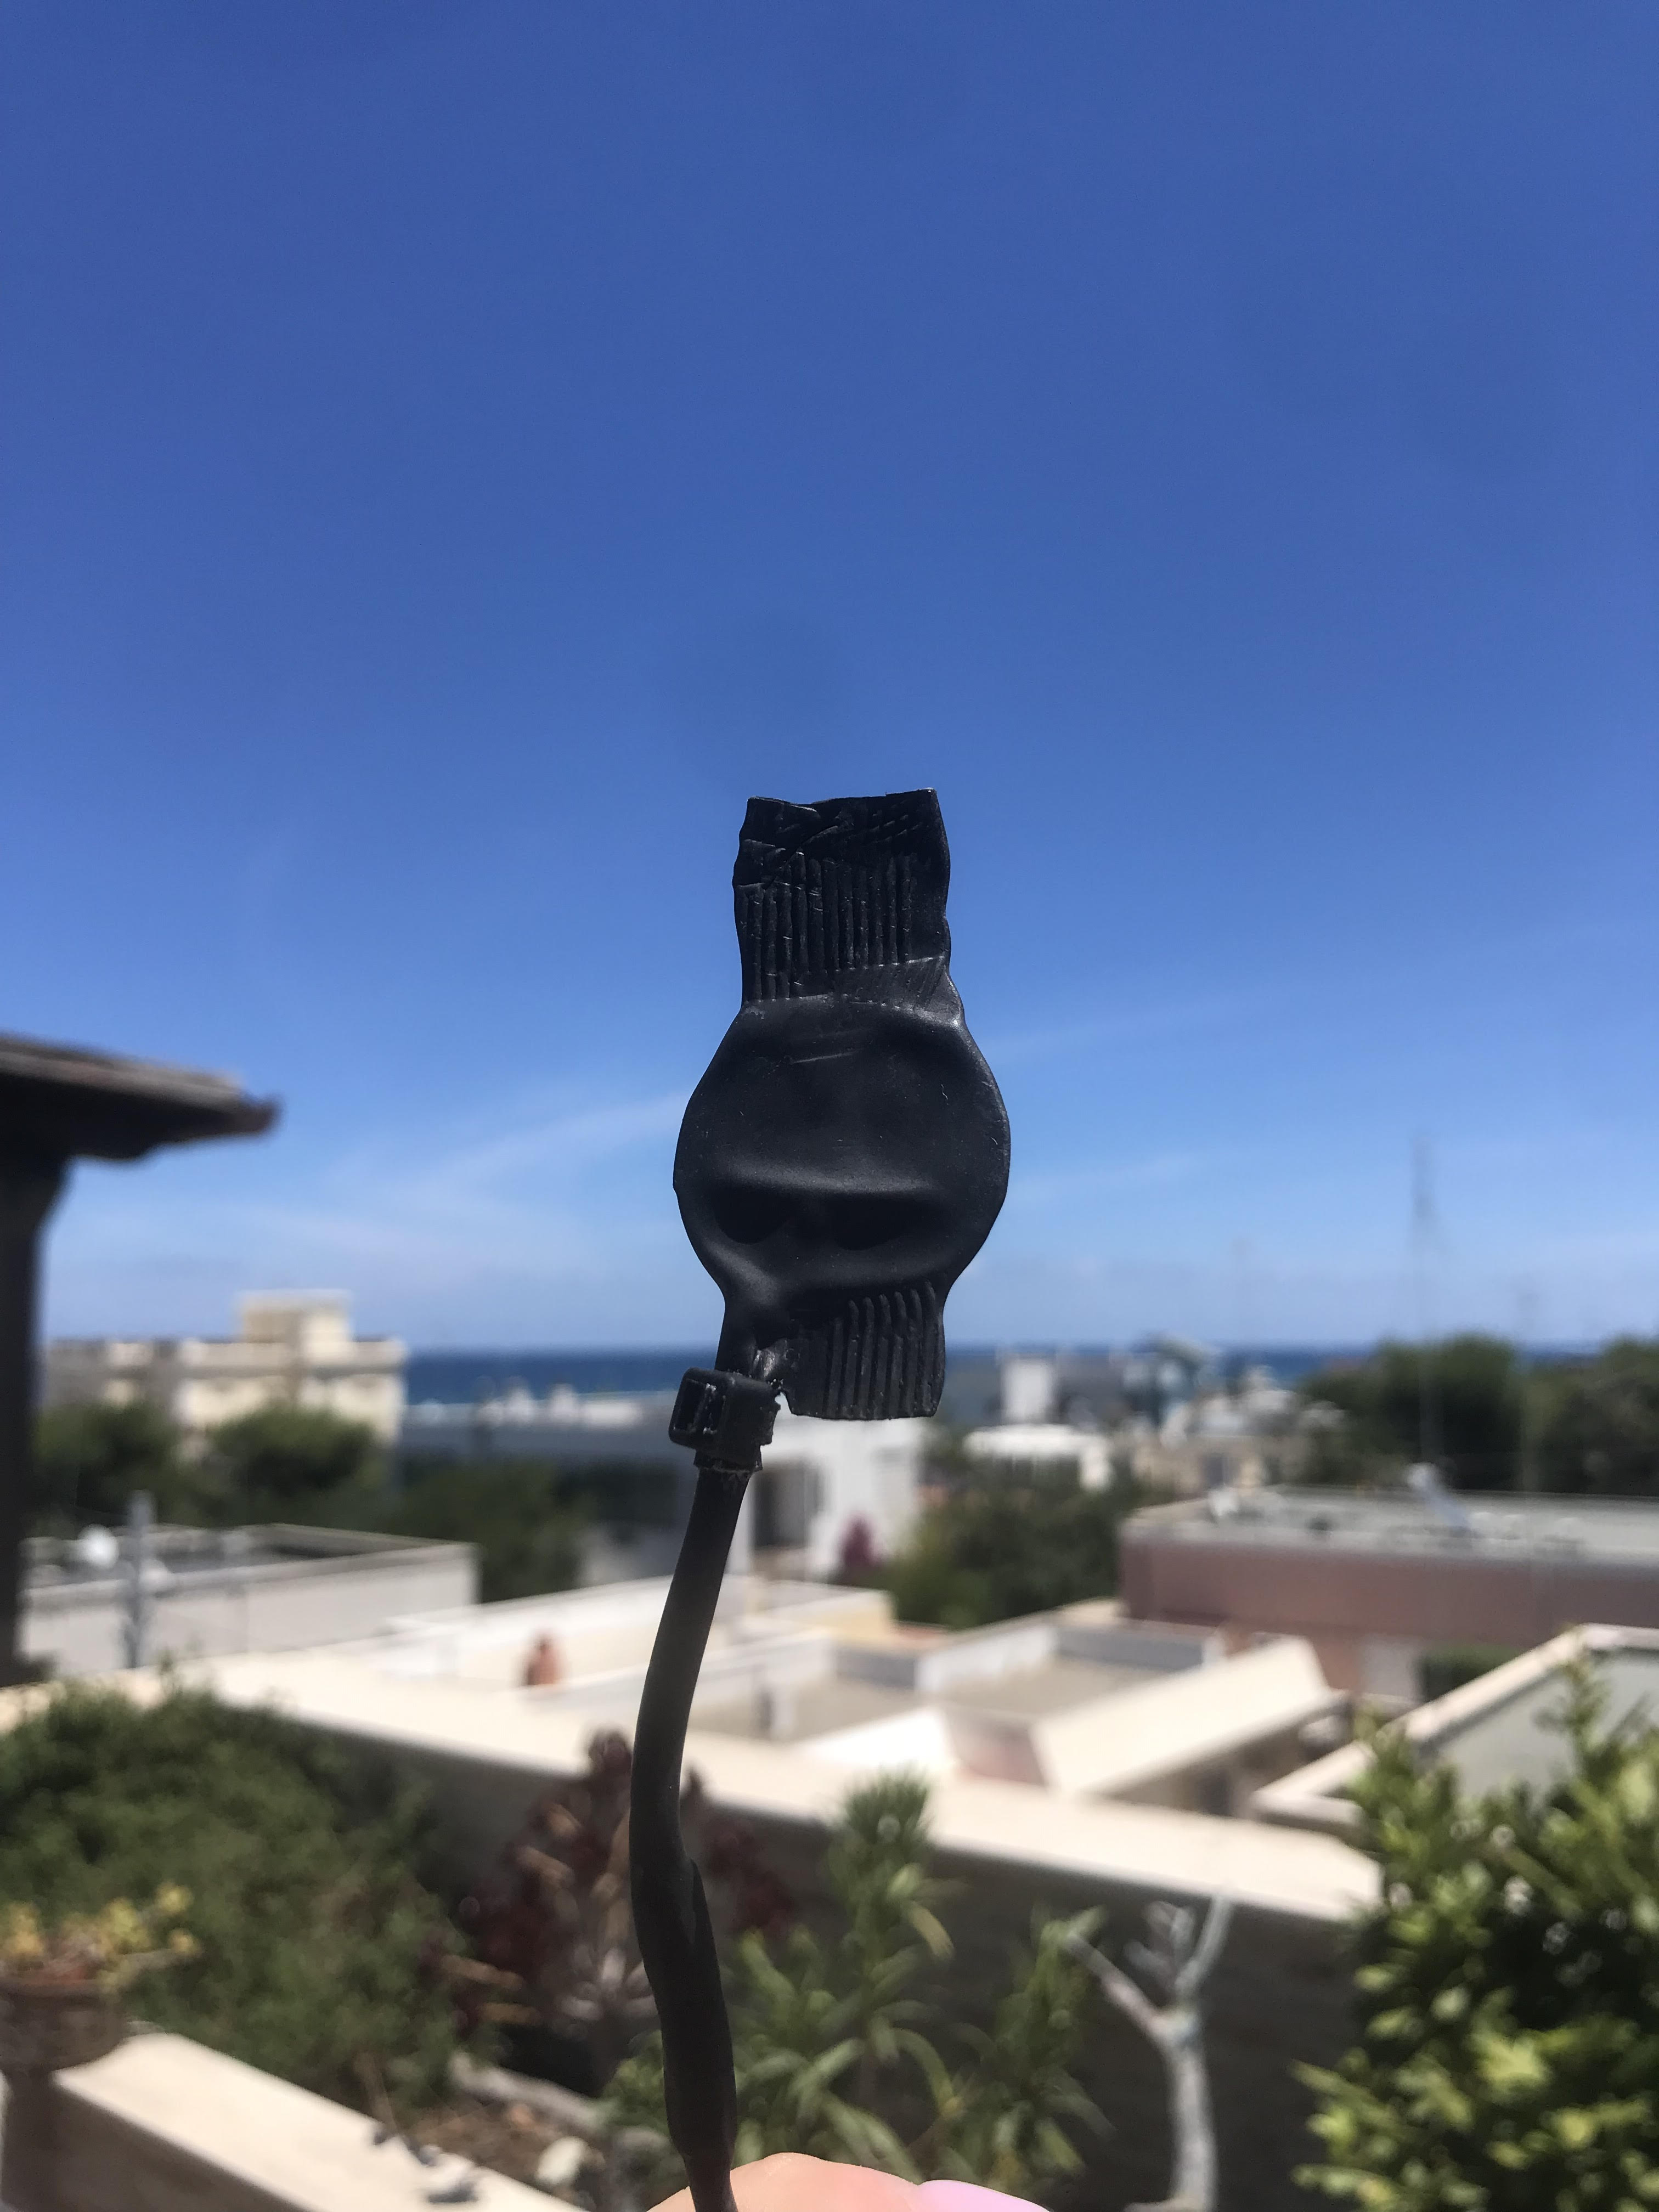
\includegraphics[width=0.9\textwidth]{foto-idro}
\caption{Idrofono realizzato...}
\end{figure}

I due piezoelettrici sono stati bilanciati , positivamente e negativamente, per poi essere collegati all'interno del cavo XLR, e isolati con della plastica, proprio per utilizzarlo nell'immersione. L' idrofono DIY (do it yourself), è stato poi sottoposto a delle registrazioni in mare. Le registrazioni sono state eseguite in due luoghi differenti, Bari Santo Spirito e Molfetta. (Figg. \ref{ressspirito,recmilitari})

\begin{figure}[h]
\centering
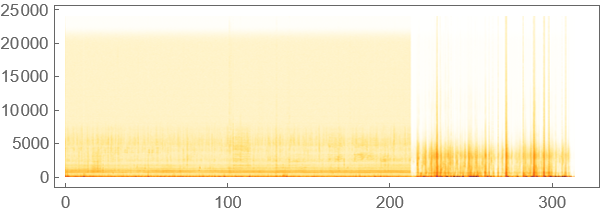
\includegraphics[width=0.9\textwidth]{164431sspiritoporto}
\caption{registrazione Porto S.Spirito}
\label{ressspirito}
\end{figure}

\begin{figure}[h]
\centering
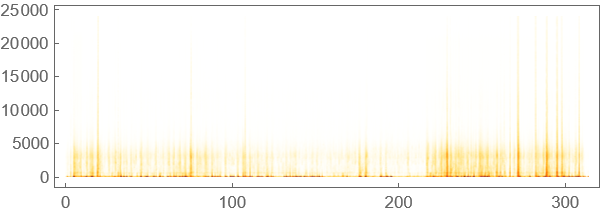
\includegraphics[width=0.9\textwidth]{173608ZonaMilitarizzata}
\caption{Idrofono realizzato...}
\label{recmilitari}
\end{figure}

Nel primo caso, le riprese effettuate hanno riscontrato suoni e rumori, provenienti da motori di barche, rigetto di reti; La maggior parte delle registrazioni hanno ripreso rumori di fondo generali, dovuti al materiale con cui è stato costruito l'idrofono. 
Nel secondo caso, le registrazioni alla profondità di 20mt, non hanno riscontrato particolare attenzione, rumori molto bassi o quasi indefinibili. 
Proprio da questi esempi, l'utilizzo di un idrofono professionale avrebbe dato sicuramente una maggiore affidabilità a quello che è tutt'oggi l'obiettivo della ricerca. Cosa davvero provoca l'inquinamento acustico? Come il rumore contribuiscea definire inquinato il nostro mare?
Nell'immaginario collettivo, spesso l'ambiente subacqueo è totalmente privo di suoni, ma nella realtà non è così. Il mondo sottomarino è tutt'altro che silenzioso, e basta immergere la testa sott'acqua qualche secondo, per scoprirlo.
Nel linguaggio comune si parla di "rumore subacqueo", ma ciò che percepiamo, anche quando semplicemente nuotiamo in apnea, non è un singolo rumore, bensì la somma di una miriade di suoni. Sono i suoni prodotti dai numerosi organismi marini, i suoni originati dagli agenti atmosferici come il rumore delle onde e del vento, che si uniscono a loro volta ai rumori generati dalle attività umane, in certi casi particolarmente invasivi.
Per questo è più corretto parlare di "clima acustico subacqueo". 
L’ambiente marino consente al suono di percorrere notevoli distanze, nell’ordine di 1500 metri in un secondo, e ciò facilita la trasmissione, oltre che di suoni biologici, anche di tutta una vasta gamma di rumori, tra cui quelli di origine antropica, riguardo ai quali la comunità scientifica muove una sempre maggiore attenzione. Questi suoni, infatti, non interferiscono unicamente con le capacità sensoriali degli animali e la loro possibilità di comunicare, ma potrebbero anche avere una gamma più estesa di effetti, dalla morte immediata allo spostamento da abituali siti di foraggiamento ed anche di alterazione del rapporto preda/predatore o dei comportamenti riproduttivi e di orientamento. 
La Commissione Europea definisce l’inquinamento acustico sottomarino come “l’introduzione intenzionale o accidentale di energia acustica nella colonna d’acqua, da fonti puntuali o diffuse”.

Viste le scarse conoscenze specifiche sui suoi potenziali effetti si applica il "principio precauzionale" secondo cui l’assenza di certezza scientifica, qualora sussista il pericolo di danni gravi o irreversibili, non esonera gli Stati dal dovere di predisporre misure efficaci per evitare il degrado ambientale.

Per il monitoraggio del rumore subacqueo vengono presi in considerazione due indicatori:
\begin{itemize}
\item i suoni impulsivi, causati principalmente da attività esplorative a fini estrattivi e l’installazione di pali per la costruzione di piattaforme e stazioni eoliche
\item i suoni continui, generati principalmente dal trasporto marittimo
\end{itemize}

Grazie all'arpa FVG, sono riuscita ad avere contatti con MARITIME TECHNOLOGY CLUSTER FVG , Il punto di riferimento per il settore delle tecnologie marittime nel Friuli Venezia Giulia,un insieme di imprese, università, centri di ricerca, enti di formazione, il quale mi ha consigliato di contattare l'Istituto Nazionale di Oceanografia e di Geofisica Sperimentale nella provincia di Trieste. 
Grazie alla dott.ssa Tinivella, docente della sezione di Geofisica, ho avuto contatti con il CIBRA “Centro Interdisciplinare di Bioacustica”. 
Il CIBRA nasce nel 1989 come “Centro Interdisciplinare di Bioacustica” grazie al Professor Mario Pavan (1918-2003), allora Direttore dell'Istituto di Entomologia, e al Magnifico Rettore Roberto Schmid. Il Centro nasce sulle esperienze del Laboratorio di Bioacustica numerica avviato nove anni prima nell’ambito del lavoro di tesi del Dott. Gianni Pavan, e si è presto affermato come laboratorio all'avanguardia anche a livello internazionale nel settore della bioacustica e della nascente disciplina della Computational Bioacoustics. In seguito, il Centro cambia denominazione e diventa “Centro Interdisciplinare di Bioacustica e Ricerche Ambientali” per meglio indicare la valenza e le applicazioni della bioacustica nel settore ambientale, in particolare per il monitoraggio e la tutela della biodiversità.
Dalle prime ricerche strettamente di bioacustica sulle caratteristiche acustiche di singole specie, terrestri e marine, si passa a ricerche di più ampio respiro che si avvicinano ai temi dell'ecologia acustica e dell'acustica ambientale, fino a partecipare alla nascita nel 2014 di una nuova disciplina, l’Ecoacustica, che coniuga appunto bioacustica ed ecologia, e alla fondazione della International Ecoacoustic Society.
Negli ultimi anni, anche a causa dei costi elevati nel mantenere ricerche in mare, l'attenzione del CIBRA si è spostata sulla bioacustica e sull’ecoacustica come strumenti di monitoraggio ambientale terrestre e marino con la rivalutazione del concetto di Paesaggio Sonoro, tema talvolta borderline rispetto al tradizionale approccio scientifico.
il dott. Claudio Fossati Docente dell'Università di Pavia, specializzato nella ricerca del rumore del fondale marino, ha contribuito e collaborato allo ricerca di questo argomento, consegnandomi dati significativi, registrazioni provenienti dal mare della Puglia, che andremo in seguito ad analizzare. 

\section{Esempi}